\section{Мета роботи}
Закріпити теоретичні знання та набути практичного досвіду
впорядкування набору статичних та динамічних структур даних.

\noindent
\textbf{Теми для попередньої роботи:}
\begin{itemize}
    \item масиви та списки;
    \item алгоритми сортування вибором та включенням;
    \item алгоритми сортування вибором на деревах, розподілом та злиттям.
\end{itemize}


\section{Завдання}
Написати програму, що реалізує три алгоритми сортування набору
даних згідно з табл. 12.1.

Визначити кількість порівнянь та обмінів для початкових наборів
даних, що містять різну кількість елементів (50, 1000, 5000, 10000, 50000).

Оцінити час сортування. Дослідити вплив початкової впорядкованості
набору даних (відсортований, відсортований у зворотному порядку,
випадковий).


\section{Хід виконання}
Для виконання завдання було обрано мову Rust.
Увесь код також додатково був розміщений в GitHub репозитарії: \href{https://github.com/blackgolyb/algos-labs}{https://github.com/blackgolyb/algos-labs}.


\newpage
\subsection{Пірамідальне сортування}
\lstinputlisting[language=Rust, style=colouredRust]{\codeDirectory/src/libs/sort/variants/heap.rs}


\newpage
\subsection{Порозрядне цифрове сортування}
\lstinputlisting[language=Rust, style=colouredRust]{\codeDirectory/src/libs/sort/variants/radix.rs}


\newpage
\subsection{«Кишенькове» сортування}
Для цього сортування додамо додаткову умову для сортованого типа.
Сортований тип повинен буде реалізовувати інтерфейс AsIndex який буде дозволяти отримати порядковий номер для кожного елемента.
\lstinputlisting[language=Rust, style=colouredRust]{\codeDirectory/src/libs/sort/variants/bucket.rs}


\newpage
\subsection{Приклад роботи програми}
\noindent
Код програми для перевірки:
\lstinputlisting[language=Rust, style=colouredRust]{\codeDirectory/src/labs/lab12/main.rs}


\begin{figure}[ht!]
    \centering
    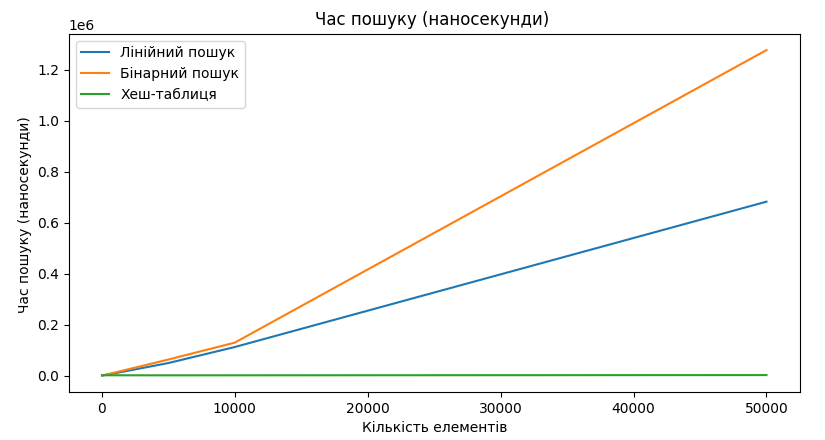
\includegraphics[width=.8\textwidth]{\assetsDirectory/time.png}
    \caption{Залежність часу пошуку від кількості елементів}
\end{figure}
\begin{figure}[ht!]
    \centering
    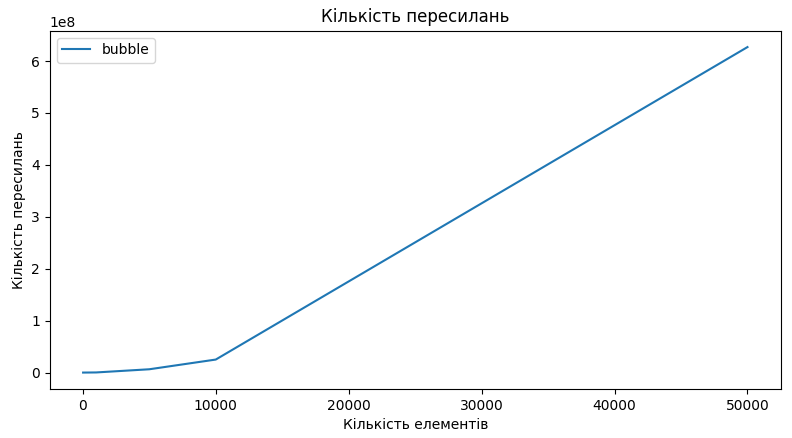
\includegraphics[width=.8\textwidth]{\assetsDirectory/swap.png}
    \caption{Залежність кількості пересилань від кількості елементів}
\end{figure}
\begin{figure}[ht!]
    \centering
    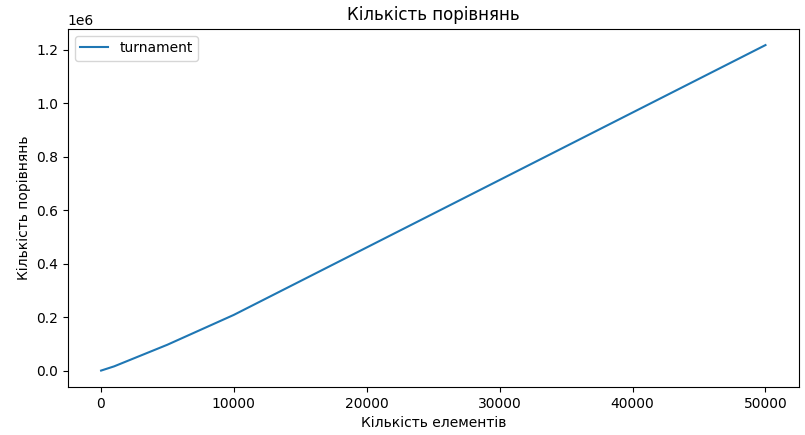
\includegraphics[width=.8\textwidth]{\assetsDirectory/comp.png}
    \caption{Залежність кількості порівнянь від кількості елементів}
\end{figure}


\newpage
\section{Висновки}
В ході виконання лабораторної робити було створено такі сортування: heap sort, radix sort, bucket sort.
Також було протестовано їх на різних обємах даних та побудовано графіки для наглядної демонстрації їх характеристик.
